% Blind, Pre-Registered Validation of LLM Population Simulation:
% A Pass, Its Mechanism, and a Falsification.
%
% v1.0 — sealed by the owner's ruling of 2026-07-21.
% Every quantitative claim is transcribed from a sealed record under runs/
% (verdict records: docs/M4_BT1_VERDICT_RECORD.md, docs/BT2_VERDICT_RECORD.md,
% docs/E7_FLATNESS_AUDIT.md) or generated from runs/e7_ess/results.json via
% figures/gen_numbers.py (% AUTO-GENERATED by figures/gen_numbers.py from runs/e7_ess/results.json
% do not edit by hand
\newcommand{\essTOneAll}{0.660}
\newcommand{\essTOneAllESS}{$\leq 10$}
\newcommand{\essTOneHold}{0.645}
\newcommand{\essTOneHoldESS}{$\leq 10$}
\newcommand{\essTTwoAll}{0.659}
\newcommand{\essTTwoAllESS}{$\leq 10$}
\newcommand{\essTTwoHold}{0.644}
\newcommand{\essTTwoHoldESS}{$\leq 10$}
\newcommand{\essTThreeAll}{0.692}
\newcommand{\essTThreeAllESS}{$\leq 10$}
\newcommand{\essTThreeHold}{0.673}
\newcommand{\essTThreeHoldESS}{$\leq 10$}
\newcommand{\essTFourAll}{0.146}
\newcommand{\essTFourAllESS}{$>5000$}
\newcommand{\essTFourHold}{0.510}
\newcommand{\essTFourHoldESS}{$\lesssim 10$}
\newcommand{\essTFourNCAll}{0.147}
\newcommand{\essTFourNCAllESS}{$>5000$}
\newcommand{\essTFourNCHold}{0.506}
\newcommand{\essTFourNCHoldESS}{$\approx 20$ ($\geq 11$)}
\newcommand{\essTFourNFAll}{0.215}
\newcommand{\essTFourNFAllESS}{$>5000$}
\newcommand{\essTFourNFHold}{0.516}
\newcommand{\essTFourNFHoldESS}{$\leq 10$}
\newcommand{\essTFiveAll}{0.097}
\newcommand{\essTFiveAllESS}{$>5000$}
\newcommand{\essTFiveHold}{0.221}
\newcommand{\essTFiveHoldESS}{$>1000$}
\newcommand{\essDeployAll}{0.114}
\newcommand{\essDeployAllESS}{$>5000$}
\newcommand{\essDeployHold}{0.216}
\newcommand{\essDeployHoldESS}{$>1000$}
\newcommand{\essTemplAll}{0.047}
\newcommand{\essTemplAllESS}{$>5000$}
\newcommand{\essTemplHold}{0.193}
\newcommand{\essTemplHoldESS}{$>1000$}
\newcommand{\essHtoHDirection}{\emph{worse}}
\newcommand{\essHtoHDelta}{0.095}
\newcommand{\essHtoHCI}{$[0.092, 0.098]$}
\newcommand{\essHtoHHoldSentence}{and remains worse by 0.054 $[0.046, 0.062]$ on the held-out target.}
\providecommand{\essNarrative}{}
\providecommand{\essFigureNote}{}
). Build: tectonic main.tex
\documentclass[11pt]{article}

\usepackage[margin=1.1in]{geometry}
\usepackage{amsmath,amssymb}
\usepackage{booktabs}
\usepackage{graphicx}
\usepackage{xcolor}
\usepackage{tcolorbox}
\usepackage{microtype}
\usepackage{enumitem}
\usepackage[hidelinks]{hyperref}
\usepackage{caption}
\usepackage[round]{natbib}
\captionsetup{font=small,labelfont=bf}

\newcommand{\dq}{\Delta Q}
\newcommand{\arena}[1]{\textsc{#1}}
% AUTO-GENERATED by figures/gen_numbers.py from runs/e7_ess/results.json
% do not edit by hand
\newcommand{\essTOneAll}{0.660}
\newcommand{\essTOneAllESS}{$\leq 10$}
\newcommand{\essTOneHold}{0.645}
\newcommand{\essTOneHoldESS}{$\leq 10$}
\newcommand{\essTTwoAll}{0.659}
\newcommand{\essTTwoAllESS}{$\leq 10$}
\newcommand{\essTTwoHold}{0.644}
\newcommand{\essTTwoHoldESS}{$\leq 10$}
\newcommand{\essTThreeAll}{0.692}
\newcommand{\essTThreeAllESS}{$\leq 10$}
\newcommand{\essTThreeHold}{0.673}
\newcommand{\essTThreeHoldESS}{$\leq 10$}
\newcommand{\essTFourAll}{0.146}
\newcommand{\essTFourAllESS}{$>5000$}
\newcommand{\essTFourHold}{0.510}
\newcommand{\essTFourHoldESS}{$\lesssim 10$}
\newcommand{\essTFourNCAll}{0.147}
\newcommand{\essTFourNCAllESS}{$>5000$}
\newcommand{\essTFourNCHold}{0.506}
\newcommand{\essTFourNCHoldESS}{$\approx 20$ ($\geq 11$)}
\newcommand{\essTFourNFAll}{0.215}
\newcommand{\essTFourNFAllESS}{$>5000$}
\newcommand{\essTFourNFHold}{0.516}
\newcommand{\essTFourNFHoldESS}{$\leq 10$}
\newcommand{\essTFiveAll}{0.097}
\newcommand{\essTFiveAllESS}{$>5000$}
\newcommand{\essTFiveHold}{0.221}
\newcommand{\essTFiveHoldESS}{$>1000$}
\newcommand{\essDeployAll}{0.114}
\newcommand{\essDeployAllESS}{$>5000$}
\newcommand{\essDeployHold}{0.216}
\newcommand{\essDeployHoldESS}{$>1000$}
\newcommand{\essTemplAll}{0.047}
\newcommand{\essTemplAllESS}{$>5000$}
\newcommand{\essTemplHold}{0.193}
\newcommand{\essTemplHoldESS}{$>1000$}
\newcommand{\essHtoHDirection}{\emph{worse}}
\newcommand{\essHtoHDelta}{0.095}
\newcommand{\essHtoHCI}{$[0.092, 0.098]$}
\newcommand{\essHtoHHoldSentence}{and remains worse by 0.054 $[0.046, 0.062]$ on the held-out target.}
\providecommand{\essNarrative}{}
\providecommand{\essFigureNote}{}
 % WS1 macros generated from runs/e7_ess/results.json

\title{\bfseries Blind, Pre-Registered Validation of LLM Population
Simulation:\\ A Pass, Its Mechanism, and a Falsification}
\author{Umar Aslam\thanks{Draft prepared with agent assistance under the
project's standing rules: agents draft, the owner seals. All blind
verdicts referenced here were sealed before this paper was written and
cannot be altered by it.}\\[2pt]
{\small Independent researcher}\\
{\small \url{https://github.com/Umaraslam66/Agora}}}
\date{July 2026 --- v1.0}

\begin{document}
\maketitle

\begin{abstract}
\noindent
LLM-based simulations of human populations are spreading faster than the
standards used to validate them. We report what we believe is the first
\emph{blind, pre-registered, adversarially controlled} validation of an
LLM population-simulation method against held-out natural experiments,
with every metric, bar, and decision rule frozen and published before
any blind quantity was scored --- and with both a positive and a negative
verdict sealed, whatever they said. The method seeds one persona per real
household-travel-diary record, executes daily choices with a calibrated
fast (non-LLM) executor governed by an LLM-written behavioral card, and
lets an LLM slow brain rewrite cards under announced policy shocks. In
the primary arena (the Seattle SR~99 tunnel tolling of 2019), the
placebo-corrected blind prediction covered the observed $-28\%$ volume
response (central drop $0.275$, 80\% interval $[0.267, 0.286]$ as
fractions of baseline volume) and beat both the official forecast
($-45\%$) and a no-LLM calibrated comparator (central $0.310$,
non-covering). A same-day mechanism audit, sealed as an
amendment before the second arena fired, showed $\geq 98.6\%$ of the
predicted response flowed through the calibrated route-choice channel and
$\approx 1\%$ through LLM card rewrites: the method won through
\emph{calibration transfer}, not runtime persona intelligence. The frozen
method was then transferred unchanged to a second blind arena (the
Stockholm congestion charge, cross-instrument and cross-population by
design). The transfer verdict is an unambiguous, clean null: the card
channel prices at $\sim 0.05\%$ of baseline against a real-world
$\sim 21\%$ effect, the pre-registered hysteresis signature fails at
every sensitivity threshold, and yoked placebo arms show the null is not
drift. A non-blind information-value analysis in equivalent-sample-size
units completes the picture at the individual level: persona cards
carrying no behavioral evidence are worth fewer than ten real diary
records at individual prediction, the value of an observed day is almost
entirely replay rather than generalization, and a deterministic template
card built from the same diary strictly outperforms the LLM-written
card. We conclude that what was
demonstrated is calibration transfer through a disciplined harness; the
LLM adaptation channel, as built, carries no measurable price response
--- and that the pre-registration harness itself, which caught all of
this, is the main contribution.
\end{abstract}

\section{Introduction}
\label{sec:intro}

Generative-agent simulation is having a moment. Since interactive
LLM-agent societies were first demonstrated \citep{park2023generative},
and especially since LLM agents seeded from interview transcripts were
shown to reproduce survey responses of a thousand real individuals
\citep{park2024thousand}, a growing body of work treats LLM populations
as instruments for social-science measurement, policy piloting, and
synthetic survey research. The validation standard in this literature
is, almost uniformly, \emph{fit to held-out survey answers of the same
kind the model was seeded on}, scored by researchers free to iterate
until the fit looks right.

The strands of work this builds on are by now well established.
\citet{argyle2023} showed that a suitably conditioned language model
reproduces the response distributions of demographically defined human
subgroups (``silicon samples''). \citet{aher2023} introduced Turing
experiments, replicating classic economic and social-psychology
studies with simulated participant samples. \citet{horton2023} treat
the LLM as a simulated economic agent --- \emph{Homo silicus} --- to be
endowed and experimented on in silico. And the agent-based-modeling
community has debated empirical validation standards for exactly this
class of simulation since well before LLMs entered it
\citep{windrum2007}.

That standard has three well-known failure modes. First, it cannot
distinguish memorized correlation from behavioral mechanism: the events
against which such simulations are validated are public and famous, and
the models were trained on descriptions of them. Second, it is not
blind: metric choice, threshold choice, and re-run decisions are made
after seeing results. Third, it rarely carries a falsification arm: a
cheap non-LLM baseline scored under identical protocol, so that the
marginal value of the LLM can be isolated rather than presumed.

This paper reports a validation exercise built to fail honestly on all
three axes, applied to a concrete, decision-relevant domain: urban
travel behavior under road pricing. The design principles were:

\begin{enumerate}[leftmargin=1.5em,itemsep=1pt]
\item \textbf{A frozen pre-registration outranks everything.} Every
metric (E1--E7), bar, decision rule, correction, and mechanism choice
was committed to a public repository before any blind quantity existed;
changes are append-only, dated amendments (A1--A8), each sealed before
the quantity it governs was scored, and \emph{pushed} before firing ---
commit dates are forgeable, push dates are not.
\item \textbf{Blind tests fire once.} Each arena's blind battery was
scored a single time against a quarantined truth series and sealed,
whatever it said. Re-runs are post-hoc by definition and cannot
overwrite a verdict.
\item \textbf{Adversarial controls.} A calibrated multinomial-logit
falsification arm for ordinary behavior; a no-LLM comparator arm for
the blind shock; a yoked, content-free placebo arm defining every
scored response as a drift-corrected difference; masking with a
versioned forbidden-token list and contamination probes for
memorization; and a measured two-leg drift rule that can flag any
verdict as drift-dominated.
\item \textbf{Negative results are product.} The pre-registration binds
the project to publish failures with the same prominence as passes;
deleting one is falsification.
\end{enumerate}

Under this harness the method passed its first blind test --- and the
harness itself then dismantled the flattering interpretation of that
pass. A sealed same-day audit showed the pass was carried by a
calibrated aggregate dial, not by runtime persona intelligence
(\S\ref{sec:bt1}); the second blind arena, constructed so that the
persona-adaptation channel had to do the work alone, returned a clean
null (\S\ref{sec:bt2}); and individual-level scoring shows the LLM card
adds no predictive value over a deterministic template built from the
same evidence (\S\ref{sec:ess}). We regard the resulting record --- one
pass with its mechanism correctly attributed, one falsification, and
the harness that forced both --- as the contribution.

\section{The method: five layers}
\label{sec:method}

The method is a pipeline of five layers; the LLM ``two-brain'' loop
that gives such systems their name is deliberately only one of them
(Figure~\ref{fig:pipeline}).

\begin{figure}[t]
\centering
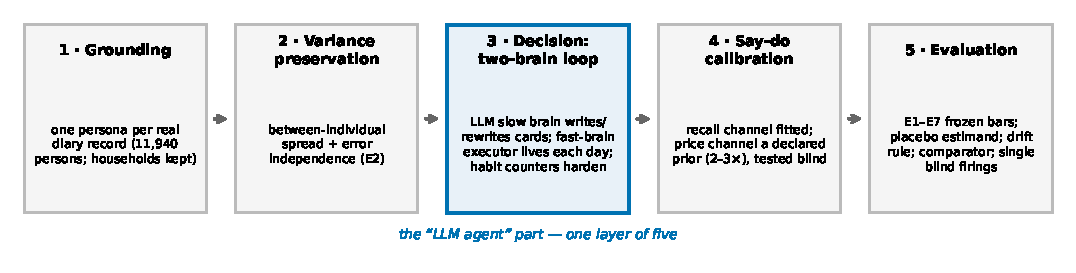
\includegraphics[width=0.95\linewidth]{figures/fig_pipeline.pdf}
\caption{The five method layers. The two-brain loop (layer 3) is one
layer of five; the blind-test mechanism audit (\S\ref{sec:bt1audit})
shows the calibrated world model of layers 1--2 and the say-do
correction of layer 4 carried the blind pass.}
\label{fig:pipeline}
\end{figure}

\paragraph{Layer 1 --- Grounding (1:1 record seeding).} Every persona
is seeded from exactly one real respondent of the Puget Sound Regional
Council household travel survey (2017 and 2019 waves; 11{,}940 persons
in 6{,}319 households), preserving the household structure. There is no
sampling from fitted marginals: each simulated person \emph{is} a
masked compression of one real person's diary, demographics, and
stated-attitude module.

\paragraph{Layer 2 --- Variance preservation.} The pipeline is scored
(eval E2) on preserving between-individual variance and error
independence --- a hidden ``single mind'' fails E2(ii) even if means are
right. Sealed result: spread ratios $0.987/1.002/0.998$ on the three
pinned dimensions (band $[0.8,1.2]$), error correlation $\approx 0$
(bar $\leq 0.20$).

\paragraph{Layer 3 --- Decision (the two-brain loop).} A \emph{slow
brain} (Qwen3-8B, temperature 0) writes a compact persona card --- day
patterns, behavioral rules, habit counters --- at initialization and
rewrites it on surprises; a \emph{fast brain} (plain code, no LLM)
executes every daily choice from the card through a calibrated
route/mode choice layer. Per-rule habit-strength counters harden with
repetition; past a calibrated threshold a rule becomes immutable and a
rewrite must restore it verbatim. Rewrites pass a five-gate validator
(schema, mask-lint, replay-smell, feasibility, fidelity-to-own-diary);
under an announced shock the fidelity gate is dropped (a gate scored
against the pre-shock diary would clamp the adaptation being measured)
and drift control moves to the placebo arm (below).

\paragraph{Layer 4 --- Say-do calibration.} Stated-vs-revealed
discrepancies are handled as two channels sealed in advance: a
\emph{recall} channel fitted person-level on stated/revealed pairs
inside the seeding data, and a \emph{price} channel declared as a
literature prior (revealed toll response $2$--$3\times$ stated;
\citealp{brownstone2005}), never fitted locally --- the pre-registration
explicitly forbids fitting it in-arena and gives it exactly one test,
the blind E3(iii) transfer clause.

\paragraph{Layer 5 --- Evaluation.} Seven eval families (E1--E7) with
frozen bars: grounding fidelity against a calibrated MNL falsification
arm (E1), variance (E2), say-do (E3), blind shock prediction (E4),
contamination probes (E5), hysteresis (E6), and an information-value
ablation (E7). The sealed E1 verdict: pooled TVD $0.0614$ (bar
$\leq 0.10$), beating the MNL arm ($0.1125$) with the paired 95\% CI of
the difference entirely below the sealed $\varepsilon=0.00655$.

\section{Study design: two blind arenas under one wall}
\label{sec:design}

\paragraph{Arenas.} The primary arena is the Seattle SR~99 tunnel
tolling event: tolling began 2019-11-09 on a tunnel with an excellent
untolled bypass; the blind window ends 2020-02-29 (pandemic cutoff).
Blind test 1 (BT1) scores the tolling onset; there is no Seattle second
test. The transfer arena is the Stockholm congestion charge
(2006 trial: on, off, permanently on), scored as blind test 2 (BT2)
with the frozen method applied unchanged. The transfer is deliberately
\emph{cross-instrument} (link toll vs.\ cordon charge),
\emph{cross-country}, and \emph{cross-population}: Stockholm personas
are the PSRC-seeded personas reweighted to published Stockholm-County
marginals (labeled \textsc{method-transfer}), a sealed design choice
that makes BT2 a test of the method rather than of source-population
idiosyncrasy --- and the amendment sealing it (A1.3) explicitly forbids
re-attributing a transfer failure to seeding class after the fact.

\paragraph{The wall.} Nothing measured after 2019-11-08 (primary) or
after the Stockholm P0 baseline (transfer) may influence any tuning,
prompt, threshold, correction, or model choice. The truth series is
import-quarantined ({\tt evaluation/truth/}) from all agent-facing code,
enforced by a static-scan plus runtime-tripwire CI test; the blind
firing entrypoints are guarded by a pre-execution hook requiring the
owner's inline authorization. Both firings were single SLURM jobs on
EuroHPC Leonardo (BT1: 10h19m; BT2: 16h02m), fired on the owner's
explicit go, with all governing amendments public before submission.

\paragraph{Masking.} Agents live in ``City K'': masked zone codes,
shifted dates, credit-denominated prices preserving per-period real
ratios, a versioned forbidden-token list (v0.3, both arenas' real
vocabulary) enforced in CI on every agent-visible byte. Contamination
probes (E5) run continuously: the masked-vs-unmasked paired A/B showed
a $4.6\%$ unmasked advantage (flag threshold $25\%$), and the
fictional-price probe showed strictly monotone price response with no
reproduction of the famous historical aggregate at non-historical
prices.

\paragraph{The placebo doctrine.} Every scored response is
$\dq = Q_{\text{policy}} - Q_{\text{placebo}}$, paired across
common-random-number ensemble members. The placebo arm yokes the
\emph{trigger} and nulls the \emph{reason}: the same agents receive, on
the same day, a content-free reconsideration notice with all price
fields nulled, in a world whose costs never change --- so a faithful
machine has nothing to do, and anything it does anyway is measured
machinery drift and subtracted. The identifying assumption (equal drift
across arms) is stated in the pre-registration as unverifiable by
design, with its known failure direction (overstating the response)
pinned before firing. A measured \emph{two-leg drift rule} guards every
verdict: a phase is flagged drift-dominated if the placebo magnitude
exceeds twice a pre-measured floor (anomaly leg) or reaches half the
policy response (absolute leg). The floors were measured and published
before each firing (primary: 0.0254 on the SR~520 rehearsal; transfer:
0.006330 on a placebo-only baseline rehearsal).

\paragraph{The comparator.} A sealed no-LLM comparator arm (A5) replays
each persona's observed diary verbatim and responds only through the
same frozen route-choice equilibrium, with its own value-of-time scale
calibrated by the same procedure on the same anchor. Its prediction was
frozen before firing: central $0.3096$, 80\% interval
$[0.2980, 0.3212]$. It is reported, never a pass bar --- with the
interpretation of either outcome pinned in advance so neither side
could be reframed post hoc.

\section{Blind test 1: the pass, and what actually carried it}
\label{sec:bt1}

BT1 fired once (submitted 2026-07-18 on the owner's explicit
authorization; run to completion and sealed 2026-07-19; Leonardo job
49744291) and scored,
together: E4 on the T5 headline population, all five E7 tiers plus the
T4-noclaims arm, the placebo arms, the tail-off bound, the comparator,
and the E6 threshold band. Frozen inputs verified at load: habit
threshold $\theta=22$, VoT scale $2.2238$, say-do price correction
$2.5\times$, drift floor $0.0254$.

\subsection{The sealed E4 verdict}

\begin{table}[h]
\centering\small
\begin{tabular}{lll}
\toprule
Sealed bar (on $\dq$, A4.2) & Value & Verdict \\
\midrule
Observed $-28\%$ inside 80\% interval & $0.28 \in [0.2673, 0.2864]$ & \textbf{PASS} \\
Central closer than the $-45\%$ forecast & $0.0048$ vs $0.1700$ & \textbf{PASS} \\
\bottomrule
\end{tabular}
\caption{BT1 headline (T5, sole headline per A4.1):
$\dq$ central $0.2752$, 80\% interval $[0.2673, 0.2864]$ against the
observed $-28\%$ tunnel-volume drop. The two-week trajectory point
($0.2798$ $[0.2651,0.2979]$ vs.\ observed $-26\%$) also covered.}
\label{tab:bt1}
\end{table}

The comparator missed: its interval $[0.2980, 0.3212]$ does not cover
$0.28$, and its central is $6\times$ farther from the observation than
the method's ($0.0296$ vs $0.0048$). The E3(iii) transfer clause ---
the frozen $2.5\times$ price correction must improve the blind central
versus the uncorrected ablation --- passed by $0.0004$ of drop:
recorded plainly as surviving its test with near-nil measured added
value in this arena. Drift verdicts: the headline arm's placebo/toll
ratio was $0.006$, four times \emph{below} the rehearsal floor;
of six populations, only T3 tripped both drift legs
(\S\ref{sec:bt1e7}).

\begin{figure}[t]
\centering
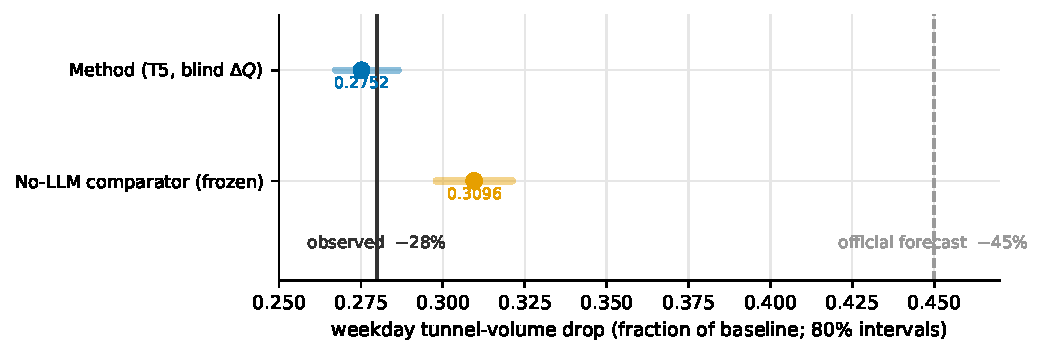
\includegraphics[width=0.85\linewidth]{figures/fig_bt1_intervals.pdf}
\caption{BT1, sealed: the method's blind 80\% interval covers the
observed $-28\%$; the frozen no-LLM comparator misses high; the
official forecast ($-45\%$) is far low. All quantities are
placebo-corrected $\dq$ per the sealed estimand.}
\label{fig:bt1}
\end{figure}

\subsection{The E7 tier curve on the blind shock}
\label{sec:bt1e7}

E7 rebuilt the full population at five nested information tiers ---
T1 demographics only, T2 $+$world context, T3 $+$stated claims,
T4 $+$one observed diary day, T5 $+$the full trace --- CRN-paired,
identical generation pipeline, plus a T4-noclaims side arm (behavior
without stated claims). All tiers fired inside the single BT1 job.

\begin{table}[h]
\centering\small
\begin{tabular}{lcccc}
\toprule
Tier & $\dq$ central & 80\% & covers $0.28$ & drift-dominated \\
\midrule
T1 & 0.2748 & [0.2673, 0.2856] & yes & no \\
T2 & 0.2741 & [0.2645, 0.2843] & yes & no \\
T3 & 0.2078 & [0.1998, 0.2171] & \textbf{no} & \textbf{YES} \\
T4 & 0.2798 & [0.2693, 0.2921] & yes & no \\
T4-noclaims & 0.2883 & [0.2772, 0.3001] & yes & no \\
T5 & 0.2752 & [0.2673, 0.2864] & yes & no \\
\bottomrule
\end{tabular}
\caption{E7 on BT1 (diagnostic; T5 is the sole headline). The curve is
flat except T3 --- and \S\ref{sec:bt1audit} explains both facts.}
\label{tab:e7bt1}
\end{table}

Two anomalies stand out: the curve is \emph{flat} (a demographics-only
tier covers the blind truth), and T4-noclaims sits \emph{above} T4
(withholding stated claims moved the central $+0.85$pp). Both were
attacked before any interpretation was allowed to stand.

\subsection{The sealed mechanism audit: dial-dominated}
\label{sec:bt1audit}

A same-day, owner-run audit (sealed as amendment A7 before the second
arena fired) decomposed every arm's response exactly into a
\emph{demand term} (corridor car-travel leaves --- the only channel card
rewrites can move) and a \emph{route term} (share shift among remaining
drivers under the shared frozen VoT dial), replaying sealed arms
deterministically (drop reproduction $<10^{-9}$; per-agent facility
reconstruction exact in 8/8 arms).

\begin{figure}[t]
\centering
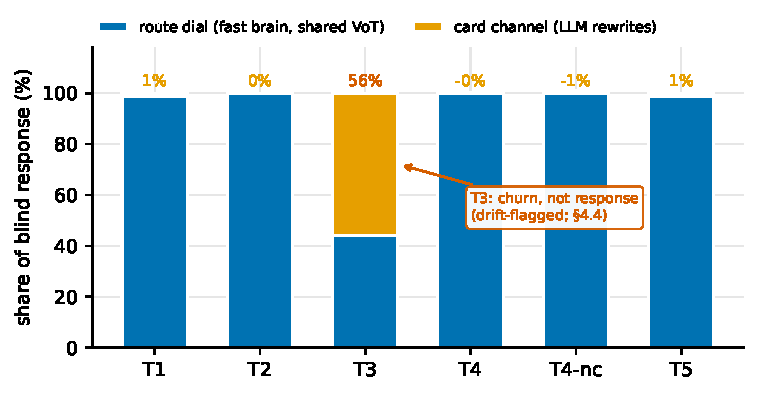
\includegraphics[width=0.9\linewidth]{figures/fig_decomposition.pdf}
\caption{The sealed two-term decomposition of the BT1 response (audit
A7): in every covering tier $\geq 98.6\%$ of $\dq$ flows through the
fast-brain route-choice dial; the card-rewrite channel carries
$\approx 1\%$. T3's anomalous split is churn, not response
(\S\ref{sec:t3}).}
\label{fig:decomp}
\end{figure}

In every covering tier at least $98.6\%$ of the scored response flows
through the fast-brain route choice under the shared calibrated dial
--- a channel that is tier-invariant by construction. The card-rewrite
channel, the only channel tier information can touch, carried
$\approx 1\%$. The tiers genuinely differ (0\% identical cards across
tiers; added-rule similarity to T5 of only 0.02--0.35), so the flat
curve is not accidental sameness: different personas produce different
adaptations, feeding a channel that carries one percent of the
response. The flat curve is arithmetic, not a discovery about
information value.

The comparative reading against the no-LLM comparator was corrected
accordingly, and the sealed amendment requires every future summary to
carry it verbatim: \emph{``the two-brain method beat the aggregate
comparator through calibration transfer --- the adaptation channel's
presence at fit time moved the dial to the right place --- not through
runtime persona intelligence.''} Concretely: the method's VoT dial was
jointly calibrated with the LLM adaptation channel present and the
say-do correction applied, landing at scale $2.2238$, which transfers
to $0.275$ at the blind rates; the comparator's solo calibration landed
at $1.8512 \to 0.310$, outside its own interval. BT1 may not be
presented as evidence that persona-level simulation adds predictive
value over a well-calibrated aggregate model in this arena.

\subsection{The T3 instability: stated claims without behavior}
\label{sec:t3}

T3 --- stated claims with no observed behavior --- is the sole
non-covering tier and the sole drift-flagged tier, and the audit showed
these are one phenomenon. Rewriting a claims-only card regresses it
toward the claims \emph{regardless of notice content}: the toll and
placebo arms produced identical card-driven outcome-class splits, and
the placebo arm alone lost $25\%$ of its corridor car-driver base
(535 $\to$ 400 drivers/day) under a notice containing nothing. CRN
pairing cancels the churn in $\dq$ almost exactly, but the churn
shrinks the toll arm's driver base by $\sim 25\%$, deflating the paired
route response proportionally ($0.275 \times 0.75 \approx 0.207
\approx$ the sealed $0.2078$). The sealed two-leg drift rule flagged
exactly this tier unaided --- the control doing precisely its job.
Claims-without-behavior cards are unstable under \emph{any} rewrite
trigger; we return to this at the individual level in \S\ref{sec:ess}.

\section{Blind test 2: the falsification}
\label{sec:bt2}

BT2 is the arena the adaptation channel could not hide in. The
Stockholm cordon instrument has \emph{no route dial by construction}:
crossing the cordon is determined by origin and destination; there is
no priced route with an unpriced twin. Whatever response exists must
run through the card channel --- mode change, suppression, re-timing.
The transfer inventory pre-declared exactly this reading, and amendment
A8 pinned the four-phase protocol (P0 baseline, P1 introduction, P2
removal --- the hysteresis phase, P3 permanent return), the yoked
placebo, the estimand, a pre-measured arena drift floor ($0.006330$,
published standalone before firing), and the requirement that the
channel decomposition ship with the verdict.

BT2 fired once (2026-07-20, Leonardo job 49860805, 16h02m) on the
owner's explicit inline authorization, after the pre-firing declaration
was pushed. The sealed verdict:

\begin{table}[h]
\centering\footnotesize
\setlength{\tabcolsep}{4pt}
\begin{tabular}{llll}
\toprule
Quantity (sealed bar) & Bar & Measured (paired $\dq$, 80\%) & Verdict \\
\midrule
P1 introduction vs truth $0.21$ & covered & $-0.00054$ $[-0.00062,-0.00048]$ & \textbf{FAIL} \\
P3 return vs truth $0.19$ & covered & $+0.00020$ $[+0.00015,+0.00026]$ & \textbf{FAIL} \\
E6 arm (a) P2 residual & $\in [0.04, 0.12]$ & $+0.000176$ $[0.000136,0.000213]$ & \textbf{FAIL} ($\sim\!200\times$ low) \\
E6 arm (b) memory-ablated & $< 0.04$ & $+0.000176$ (identical to $\sim 10^{-13}$) & vacuous \\
E6 non-overlap & intervals disjoint & identical & \textbf{FAIL} \\
E6 threshold band $\{6..26\}$ & per threshold & $\dq$ identical at every $\theta$ & \textbf{FAIL at all} \\
Drift P1/P2/P3 & $\leq 2\times 0.006330$, $<0.5$ & $0.00647/0.00651/0.00599$ & \textbf{CLEAN} \\
\bottomrule
\end{tabular}
\caption{BT2, sealed (all quantities \textsc{method-transfer}-labeled):
the method's blind response in the cordon arena is null --- three
orders of magnitude below every bar --- and the null is clean, with the
drift control green in all phases.}
\label{tab:bt2}
\end{table}

\begin{figure}[t]
\centering
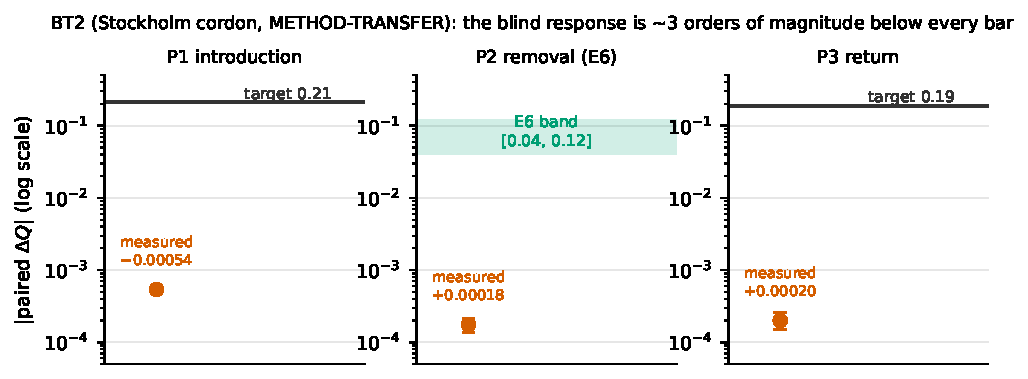
\includegraphics[width=0.9\linewidth]{figures/fig_bt2_null.pdf}
\caption{BT2, sealed: measured paired $\dq$ per phase (note the
magnified scale) against the pre-registered targets and the E6 band.
The response is $\sim 200$--$400\times$ smaller than required; placebo
magnitudes sit at the pre-measured floor, so the null is not drift.}
\label{fig:bt2}
\end{figure}

\paragraph{What the null is made of.} Every crossing agent received and
processed the announcements (3{,}999 accepted rewrites per arm-run,
charged and placebo alike). The memory-ablated arm's unconstrained
rewrites churned behavior substantially ($\sim 3.5\%$ raw drops) ---
but \emph{identically} under the priced and the nulled notice, so
pairing cancelled it: churn, not response. E6's pre-registered
contingency reading applies verbatim: arm (a) $\approx$ arm (b)
$\Rightarrow$ ``memory not load-bearing'' --- there is no hysteresis
because there is no response for habit memory to preserve. The A8.4
decomposition confirmed the pre-declared \emph{form} (share terms equal
across arms within CRN noise) while the demand terms carry no
separation because none exists. The card channel, isolated at last,
prices at $\sim 0.05\%$ of baseline against the real-world
$\sim 21\%$.

\paragraph{Reading the two verdicts together.} BT1's mechanism audit
said the response ran through the dial; BT2, an arena with no dial,
measured what the cards do alone: nothing. The A7 mechanism reading is
thereby blind-confirmed from the opposite side. A method whose BT1 pass
had genuinely run through persona adaptation would have moved here; it
did not. The falsification is clean, pre-registered, and stands sealed
beside the pass with equal prominence --- which is exactly what the
harness was built to guarantee.

\section{Information value at the individual level:\\ the E7 ordinary-day ESS analysis}
\label{sec:ess}

The blind results measure aggregates. The remaining pre-registered E7
analysis (A4.1; non-blind, scored after both arenas sealed) asks the
individual-level question: \emph{how much does each increment of
persona evidence help predict a real person's own diary days} ---
scored in equivalent-sample-size (ESS) units \citep{gao2026ess}: tier
$k$'s cards are worth $\mathrm{ESS}(k)$ real diary records if a
flexible baseline trained on that many records matches their per-person
predictive loss. The per-persona loss adapter, the baseline (the E1 MNL
arm's day-structure and mode-choice components, refit per training
block), the candidate grid, and both scoring targets were pinned in the
E7 manifest before any ESS quantity was computed. The per-persona loss
is the mean TVD, over the three frozen E1 families, between the arm's
ensemble-predicted distributions and the persona's own observed days
--- on two targets: \emph{all days} (identical across tiers; for
behavior-carrying tiers partly in evidence, i.e.\ compression), and
\emph{held-out days} (multi-day personas only, excluding the pinned
T4-shown day; a true generalization test for T4).

\begin{table}[h]
\centering\small
\begin{tabular}{lcccc}
\toprule
Arm & loss (all days) & ESS (all days) & loss (held-out) & ESS (held-out) \\
\midrule
T1 (demographics)      & \essTOneAll   & \essTOneAllESS   & \essTOneHold   & \essTOneHoldESS \\
T2 ($+$context)        & \essTTwoAll   & \essTTwoAllESS   & \essTTwoHold   & \essTTwoHoldESS \\
T3 ($+$stated claims)  & \essTThreeAll & \essTThreeAllESS & \essTThreeHold & \essTThreeHoldESS \\
T4 ($+$one day)        & \essTFourAll  & \essTFourAllESS  & \essTFourHold  & \essTFourHoldESS \\
T4-noclaims            & \essTFourNCAll & \essTFourNCAllESS & \essTFourNCHold & \essTFourNCHoldESS \\
T4-nofidelity          & \essTFourNFAll & \essTFourNFAllESS & \essTFourNFHold & \essTFourNFHoldESS \\
T5 (full trace)        & \essTFiveAll  & \essTFiveAllESS  & \essTFiveHold$^{\dagger}$ & \essTFiveHoldESS$^{\dagger}$ \\
\midrule
Deployed (M2) cards    & \essDeployAll & \essDeployAllESS & \essDeployHold$^{\dagger}$ & \essDeployHoldESS$^{\dagger}$ \\
Template cards         & \essTemplAll  & \essTemplAllESS  & \essTemplHold$^{\dagger}$ & \essTemplHoldESS$^{\dagger}$ \\
\bottomrule
\end{tabular}
\caption{E7 ordinary-day scoring at the individual level (11{,}940
personas; held-out target on the 2{,}975 multi-day personas). Loss =
mean per-persona TVD (lower is better); ESS = equivalent real diary
records (plugin / one-sided 95\% lower bound). $^{\dagger}$held-out
days in evidence for these arms (flagged per the pinned adapter).}
\label{tab:ess}
\end{table}

\begin{figure}[t]
\centering
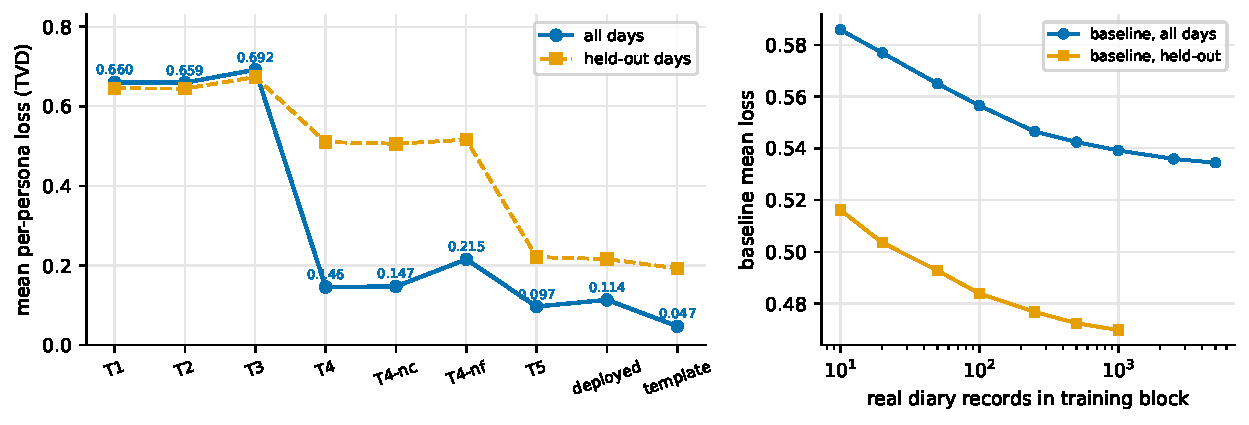
\includegraphics[width=0.95\linewidth]{figures/fig_ess_curve.pdf}
\caption{Individual-level information value. Left: mean per-persona
loss by arm on both targets. Right: the flexible baseline's learning
curve --- it flattens near $0.53$ (all days) / $0.47$ (held-out), far
above every behavior-carrying arm: no amount of \emph{other people's}
records substitutes for a person's own observed behavior, which is why
the behavior-carrying arms exceed the ESS grid on the compression
target.}
\label{fig:ess}
\end{figure}

The curve answers the individual-level question in three sharp
statements. \textbf{First: without the person's own behavior, cards
are worth less than ten strangers' records.} T1--T3 sit at losses of
$0.66$--$0.69$ against a 10-record baseline at $0.59$; the pinned
sequential test hands all three an ESS of $\leq 10$ on both targets ---
and stated claims make the card \emph{worse} than demographics alone
(T3 $0.692$ vs T1 $0.660$), the individual-level face of the T3
instability the blind test flagged (\S\ref{sec:t3}).
\textbf{Second: the value of behavioral evidence is almost entirely
compression, not generalization.} On the all-days target the
behavior-carrying arms are worth more than the entire grid ($>5{,}000$
records --- unsurprising and flagged: their evidence contains the
scored days, and the baseline's learning curve flattens near $0.53$,
so no training size reaches them). But on genuinely held-out days the
one-shown-day card collapses from $0.146$ to $0.510$, worth
$\lesssim 10$ records --- statistically indistinguishable from a
baseline trained on ten strangers --- and withholding the stated-claims
module \emph{improves} generalization (T4-noclaims $\approx 20$
records, the only tier that resolves above the grid floor). Knowing
one of a person's days buys near-nothing about their other days beyond
what population statistics already provide.
\textbf{Third: the fidelity gate, not the LLM, carries a large share
of the behavioral tiers' value.} Switching the generation-time
fidelity gate off (T4-nofidelity) degrades the loss from $0.146$ to
$0.215$ and the aggregate TVD from $0.047$ to $0.115$ --- consistent
with the sealed M2 measurement of the gate's worth ($\approx 0.07$
TVD), and further evidence that the verification machinery around the
model, not the model's authorship, does the work.

Two cross-checks anchor the analysis to the sealed record: the
deployed-population aggregate diagnostic reproduces the sealed E1
verdict to $10^{-4}$ (pooled TVD $0.0613$ here vs the sealed
$0.0614$), and the tier populations are byte-identical (SHA-256) to
those fired in BT1. The aggregate diagnostic also yields the starkest
dial-domination exhibit in the project: \textbf{T1's ordinary-day
aggregate TVD is $0.68$ --- seven times the E1 bar; as a deployed
population it would fail E1 outright --- yet its blind $\dq$ covered
the observed $-28\%$} (Table~\ref{tab:e7bt1}), because the paired,
CRN-matched estimand rides entirely on the shared calibrated dial.
Coverage of the blind aggregate was never evidence of persona realism.

\paragraph{Template vs.\ LLM head-to-head.} The deployed population
contains 8{,}496 LLM-written cards and 3{,}444 deterministic template
(fallback) cards; a full template population exists for every persona.
Paired per-persona on the 8{,}496 LLM-card personas, the LLM card is
\essHtoHDirection\ than the template card by \essHtoHDelta\ mean loss
(household-atomic bootstrap 95\% CI \essHtoHCI) on the all-days target
\essHtoHHoldSentence\ This mirrors, at the individual level, the sealed
M3 aggregate diagnostic (template pooled TVD $0.043$ vs LLM $0.074$)
--- and completes the arc of \S\ref{sec:bt1audit} and \S\ref{sec:bt2}:
at no level of analysis did the LLM's authorship of the behavioral card
demonstrate measurable predictive value beyond the evidence it was
handed.

\section{Two agents, up close}
\label{sec:walkthrough}

\begin{tcolorbox}[colback=gray!4,colframe=black!40,title={\textbf{Boxed
case study: one honest adapter, one churner} (both real, from the
sealed BT1 inspector export; masked vocabulary verbatim)},fonttitle=\small\bfseries,left=1mm,right=1mm]
\small
\textbf{P05036 (T5, full information).} A suburban two-car household's
main driver; every observed trip by car. Its card: two patterns
(commute/errand day) and two rules --- ``work $\to$ car'', ``home $\to$
car''. Both rules crossed the immutability threshold weeks before the
shock. On announcement day the slow brain rewrote the card; the entire
diff re-timed the work departure from night to the morning peak; the
locked rules came back verbatim. Over 63 charged days the policy twin
and the placebo twin differed on \emph{four} days --- all route
choices, priced crossing vs.\ parallel road. Multiply that handful of
nudged days across thousands of drivers and you get the $\approx 1\%$
card channel of the sealed audit --- visible, sensible, small.

\medskip
\textbf{P00169 (T3, claims only).} The same kind of record, but its
card was written from stated claims alone (``I usually commute by
transit''), no diary. On announcement day \emph{both} arms' rewrites
simplified the two transit rules by dropping their ``work'' qualifier
--- turning ``I take transit to work'' into ``I take transit at peak,
whatever I'm doing.'' With no behavioral anchor, the gate had nothing
to hold the card against. The twins' 102-day timelines are
byte-identical: the ``response'' to the charge equals the response to
a notice containing nothing. Hundreds of T3 agents did the same, in
both arms --- which is why T3, alone, was flagged by its own placebo.
\end{tcolorbox}

One agent with full information adapts believably and barely; one with
only self-description ``adapts'' identically no matter what it is told
--- noise wearing the costume of a response, caught by the control.
This is the information-value result in miniature: behavioral detail
earns its keep as an \emph{anchor against churn}; the method's measured
intelligence lives in its calibrated daily choices, not in dramatic
persona rewrites.

\section{Limitations}
\label{sec:limits}

Sealed caveats are restated here as the records require; none is
implicated in either verdict's direction.

\begin{enumerate}[leftmargin=1.5em,itemsep=2pt]
\item \textbf{Two arenas.} $n=2$ blind batteries, one instrument each.
The corridor arena is nearly a pure route-choice problem (the
$\approx 1\%$ card channel is a statement about that estimand, not
about persona loops generally); the cordon arena isolates the card
channel completely. Other estimands (long-run equilibria, land use,
non-price policies) are untested.
\item \textbf{\textsc{method-transfer} seeding.} Stockholm personas are
PSRC-seeded and reweighted to published marginals --- the sealed,
deliberately harder claim. The child-share rider is restated verbatim:
\emph{``children are unconstrained by M1 and follow their households;
weighted child share 13.7\% vs arena 21.9\% (2005). Expected direction
of bias: mode-share composition (escort travel, within-household car
allocation in the baseline crossing mix), \textbf{not} the price
response --- the priced adaptation channel runs through adult
decision-makers under the frozen constants, which reweighting never
touches.''}
\item \textbf{Truth-side caveats.} The Stockholm P2 anchor carries the
published roadwork confound (\emph{``off-year residual partially
confounded by roadwork at two bridges''}), which is why the E6 band was
widened $\pm 2$pp at sealing; the BT1 $-28\%$ carries an unquantified
seasonal component the placebo cannot correct (pinned pre-firing). The
measured BT2 miss ($\sim 200\times$ below band) dwarfs both.
\item \textbf{Population-margin approximations, sealed with the build:}
the M2 central-cell proxy (40.8\% $\to$ rings \{core, inner\}); M5
income excluded from raking (rank-preserving no-op without an invented
currency mapping); the masked daily charge cap recorded, not enforced
(binds only at $\geq 4$ peak crossings/day).
\item \textbf{Say-do price prior untested by transfer.} E3(iii) passed
in BT1 by $0.0004$ --- near-nil measured value --- and its transfer
reading was \emph{mooted} by the BT2 null (with the card channel inert,
the correction had no channel to act on): recorded as mooted, not
answered.
\item \textbf{ESS caveats.} The ordinary-day ESS analysis is non-blind
(scored after both arenas sealed, protocol pinned before scoring); for
behavior-carrying tiers the all-days target is partly in evidence
(compression, not generalization --- the held-out target exists for
exactly this reason); the household-atomic block adaptation to the
pinned estimator is reported with realized block sizes.
\item \textbf{One model.} The slow brain is a single 8B open-weights
model at temperature 0. Larger or different models might write cards
that price-respond; the harness is indifferent --- any such claim would
require a new pre-registered arena, and the sealed verdicts here cannot
be revised by one.
\end{enumerate}

\section{Conclusions}
\label{sec:conclusions}

Three findings, in the order the evidence forces them:

\begin{enumerate}[leftmargin=1.5em,itemsep=2pt]
\item \textbf{What was demonstrated is calibration transfer.} A
grounded, variance-preserving population with a jointly calibrated
choice dial predicted a blind natural experiment correctly and beat
both the official forecast and a no-LLM comparator --- because the
adaptation channel's presence \emph{at fit time} moved the dial to the
right place. That is a real, useful, replicable result about building
forecasting systems --- and it is not persona intelligence.
\item \textbf{The adaptation channel, as built, was falsified.} Given
an arena where only the cards could respond, they did not (0.05\% of
baseline against a 21\% real effect), at every habit threshold, with
clean controls. LLM card-rewriting under announced price shocks, in
this implementation, does not carry a price response --- and
stated-claims-only personas are actively unstable, churning identically
under signal and placebo.
\item \textbf{The harness is the contribution.} Every load-bearing
correction in this paper --- the mechanism reattribution, the T3 flag,
the falsification, the mooted prior --- was forced by machinery
committed before results existed: frozen bars, single firings, yoked
placebos, measured drift floors, adversarial comparators, quarantined
truth, and negative-results-as-product. None of it would have surfaced
under fit-to-held-out-surveys validation. We commend the harness, not
the method, to the field: the interesting question is not whether LLM
populations can fit data they have seen, but what survives when they
are made to predict, once, blind, against controls built to catch
exactly the failure that occurred.
\end{enumerate}

\subsection*{Reproducibility}

The pre-registration (with all eight amendments), the guard hooks, the
masking gates, the eval harness, both sealed verdict records, the
mechanism audit, and every number in this paper are in the public
project repository, \url{https://github.com/Umaraslam66/Agora}; blind
quantities are reproducible from the sealed {\tt runs/} manifests
(results SHA-256 pinned at firing).

\subsection*{Data availability}

The seeding microdata are the Puget Sound Regional Council household
travel survey (2017 and 2019 waves), openly downloadable from PSRC.
The truth series --- SR~99 tunnel volumes and the official forecast,
and the Stockholm phase effects --- are taken from the cited published
sources \citep{wsdot,eliasson2009,borjesson2012,eliasson2014}.
Record-derived persona cards and household-level microdata are
excluded from the repository by the project's privacy discipline
(masking gates and the no-microdata rule).

\begin{thebibliography}{99}
\small

\bibitem[Park et al.(2023)]{park2023generative}
Park, J.~S., O'Brien, J., Cai, C.~J., Morris, M.~R., Liang, P., and
Bernstein, M.~S. (2023).
Generative agents: Interactive simulacra of human behavior.
\emph{Proc.\ UIST 2023}.

\bibitem[Park et al.(2024)]{park2024thousand}
Park, J.~S., Zou, C.~Q., Shaw, A., Hill, B.~M., Cai, C.~J., Morris,
M.~R., Willer, R., Liang, P., and Bernstein, M.~S. (2024).
Generative agent simulations of 1{,}000 people.
\emph{arXiv:2411.10109v1}. (Retitled ``LLM Agents Grounded in
Self-Reports Enable General-Purpose Simulation of Individuals'' in
later revisions.)

\bibitem[Argyle et al.(2023)]{argyle2023}
Argyle, L.~P., Busby, E.~C., Fulda, N., Gubler, J.~R., Rytting, C.,
and Wingate, D. (2023).
Out of one, many: Using language models to simulate human samples.
\emph{Political Analysis}, 31(3), 337--351.

\bibitem[Aher et al.(2023)]{aher2023}
Aher, G.~V., Arriaga, R.~I., and Kalai, A.~T. (2023).
Using large language models to simulate multiple humans and replicate
human subject studies.
\emph{Proc.\ ICML 2023} (PMLR 202).

\bibitem[Horton et al.(2023)]{horton2023}
Horton, J.~J., Filippas, A., and Manning, B.~S. (2023).
Large language models as simulated economic agents: What can we learn
from \emph{Homo silicus}?
\emph{NBER Working Paper} 31122 (rev.\ February 2026);
arXiv:2301.07543.

\bibitem[Windrum et al.(2007)]{windrum2007}
Windrum, P., Fagiolo, G., and Moneta, A. (2007).
Empirical validation of agent-based models: Alternatives and
prospects.
\emph{Journal of Artificial Societies and Social Simulation}, 10(2),
8.

\bibitem[Gao et al.(2026)]{gao2026ess}
Gao, W., Han, S., and Liang, A. (2026).
How well do LLMs predict human behavior? A measure of their pretrained
knowledge.
\emph{arXiv:2601.12343}. (Equivalent-sample-size estimator pinned by
amendment A4.1; block-out CV and sequential inference used exactly as
published.)

\bibitem[Brownstone and Small(2005)]{brownstone2005}
Brownstone, D., and Small, K.~A. (2005).
Valuing time and reliability: assessing the evidence from road pricing
demonstrations.
\emph{Transportation Research Part A}, 39(4), 279--293.

\bibitem[Eliasson et al.(2009)]{eliasson2009}
Eliasson, J., Hultkrantz, L., Nerhagen, L., and Smidfelt Rosqvist, L.
(2009).
The Stockholm congestion-charging trial 2006: Overview of effects.
\emph{Transportation Research Part A}, 43(3), 240--250.

\bibitem[B{\"o}rjesson et al.(2012)]{borjesson2012}
B{\"o}rjesson, M., Eliasson, J., Hugosson, M.~B., and Brundell-Freij,
K. (2012).
The Stockholm congestion charges --- 5 years on. Effects,
acceptability and lessons learnt.
\emph{Transport Policy}, 20, 1--12.

\bibitem[Eliasson(2014)]{eliasson2014}
Eliasson, J. (2014).
The Stockholm congestion charges: an overview.
\emph{CTS Working Paper} 2014:7.

\bibitem[WSDOT(2018--2021)]{wsdot}
Washington State Department of Transportation / Washington State
Transportation Commission.
SR~99 tunnel tolling: pre-tolling forecast, rate adoption (2018-10-16),
and one-year tolling report; SR~520 toll traffic and revenue records.
Institutional sources pinned, with the reading most favorable to the
forecast, in the public pre-registration (\S7, A1.1/A3.3).

\end{thebibliography}

\end{document}
